\documentclass[es,apuntes]{uah}

\tema{3}
\titulo{Técnicas de acceso al medio}{Lesson title}
%
\begin{document}

\titulacion{Optativa GIEC y GIT}
\departamento{Teoría de la Señal y Comunicaciones}
\asignatura{Comunicaciones Digitales}{}
\curso{2021/2022} % Do not show year

\maketitle


%%%%%%%%%%%%%%%%%%%%%%%
\section{Introducción}
%%%%%%%%%%%%%%%%%%%%%%%

Cualquier sistema de comunicación se caracteriza por disponer de unos recursos escasos. Ancho de banda, potencia y número de portadoras disponibles van a estar limitados, y nuestro objetivo será sacarles el mayor partido posible.

Nos podemos plantear qué pasaría si varios usuarios desean acceder a estos recursos, como sucede por ejemplo en una red de comunicaciones móviles. Resulta evidente que deberemos dividir los recursos, y se nos pueden ocurrir al menos tres formas de hacerlo:

\begin{itemize}
	\item {\bf División en frecuencia}: Asignar una banda de frecuencia distinta a cada usuario.
	\item {\bf División en tiempo}: Asignar un slot temporal a cada usuario.
	\item {\bf División por código}: Asignar un código distinto para la comunicación a cada usuario. 
\end{itemize}

Por ejemplo, si realizamos un estudio de las distintas técnicas de acceso al medio utilizadas en los distintos estándares de telefonía móvil, nos encontramos con lo siguiente:

\begin{itemize}
	\item {\bf 1G}: FDMA (\textit{Frequency Division Multiple Access}).
	\item {\bf 2.xG}: TDMA (\textit{Time Division Multiple Access}) (o combinaciones de SDMA (\textit{Spatial Division Multiple Access}) con TDMA)
	\item {\bf 3.xG}: W-CDMA (\textit{Code Division Multiple Access})
	\item {\bf 4G}: OFDMA (\textit{Orthogonal Frequency Division Multiple Access}) + MIMO 
\end{itemize}

Lo que haremos a continuación es ir repasando cada una de estas técnicas con algo más de detalle. 


%%%%%%%%%%%%%%%
\section{FDMA (\textit{Frequency Division Multiple Access})}\index{FDMA}\index{Frequency Division Multiple Access}
%%%%%%%%%%%%%%%

Los sistemas FDMA se basan en dividir el ancho de banda total en un cierto número de canales, separados generalmente entre sí con una cierta banda de guarda. A cada usuario se le asignan después uno o varios canales, que serán los que pueda utilizar para sus comunicaciones. 

La Figura \ref{fig:FDMA} muestra de forma gráfica cómo se organiza la información de los distintos usuarios en un sistema FDMA. 


\begin{figure*}[h!]
	\centering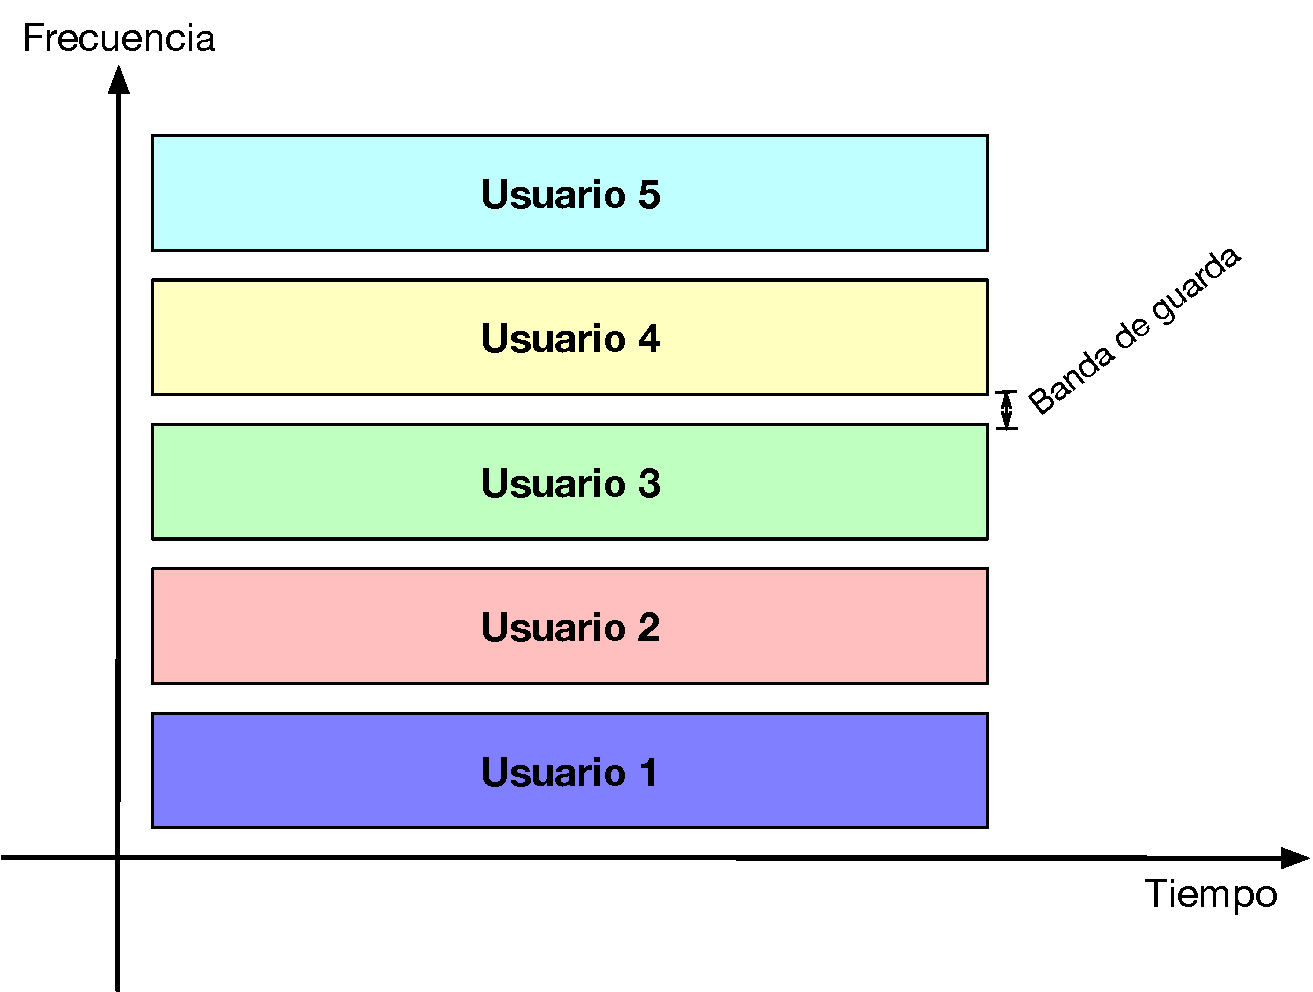
\includegraphics[width=8cm]{./Figuras/FDMA}
	\caption{Sistema FDMA.}
	\label{fig:FDMA}
\end{figure*}
	
	
Podemos citar como ventajas de este tipo de sistemas:

\begin{itemize}
	\item Son compatibles con modulaciones tanto analógicas como digitales.
	\item La implementación de los equipos es muy sencilla.
\end{itemize}

Por contra, los principales inconvenientes de los sistemas FDMA son:

\begin{itemize}
	\item No aprovecha bien el espectro disponible, en comparación con otros sistemas como TDMA o CDMA. 
	\item Son sistemas rígidos, con dificultad para adaptarse a diferentes aplicaciones o flujos de datos. 
	\item La interferencia entre subcanales puede causar problemas, al colarse la señal de un canal en otro canal adyacente.
\end{itemize}

Entre las aplicaciones de este tipo de sistemas podemos citar la FM comercial, donde cada emisora de radio tiene asignado su canal de transmisión, o la transmisión por fibra óptica, aunque en este caso se tiene a hablar más de WDMA (\textit{Wavelength Division Multiple Access}). En el caso de la radio FM comercial en España, por ejemplo, se utilizan canales con un ancho de banda de $150kHz$ y una banda de guarda de $25kHz$ a cada lado. 

%%%%%%%%%%%%%%%
\section{TDMA}\index{TDMA}\index{Time Division Multiple Access}
%%%%%%%%%%%%%%%

Los sistemas TDMA lo que hacen es asignar todo el ancho de banda a todos los usuarios pero éstos sólo pueden transmitir durante unos determinados \emph{slots} de tiempo que tienen asignados, nunca de forma simultánea. Así, cada cliente transmite su información de forma discontinua, en forma de ráfagas o \emph{bursts} de información en cada \emph{slot}, que en general son sólo una pequeña porción de todo lo que pretenden transmitir. 

En la Figura \ref{fig:TDMA} se muestra la forma de organizar la información de distintos usuarios en un sistema TDMA. 

\begin{figure*}[h!]
	\centering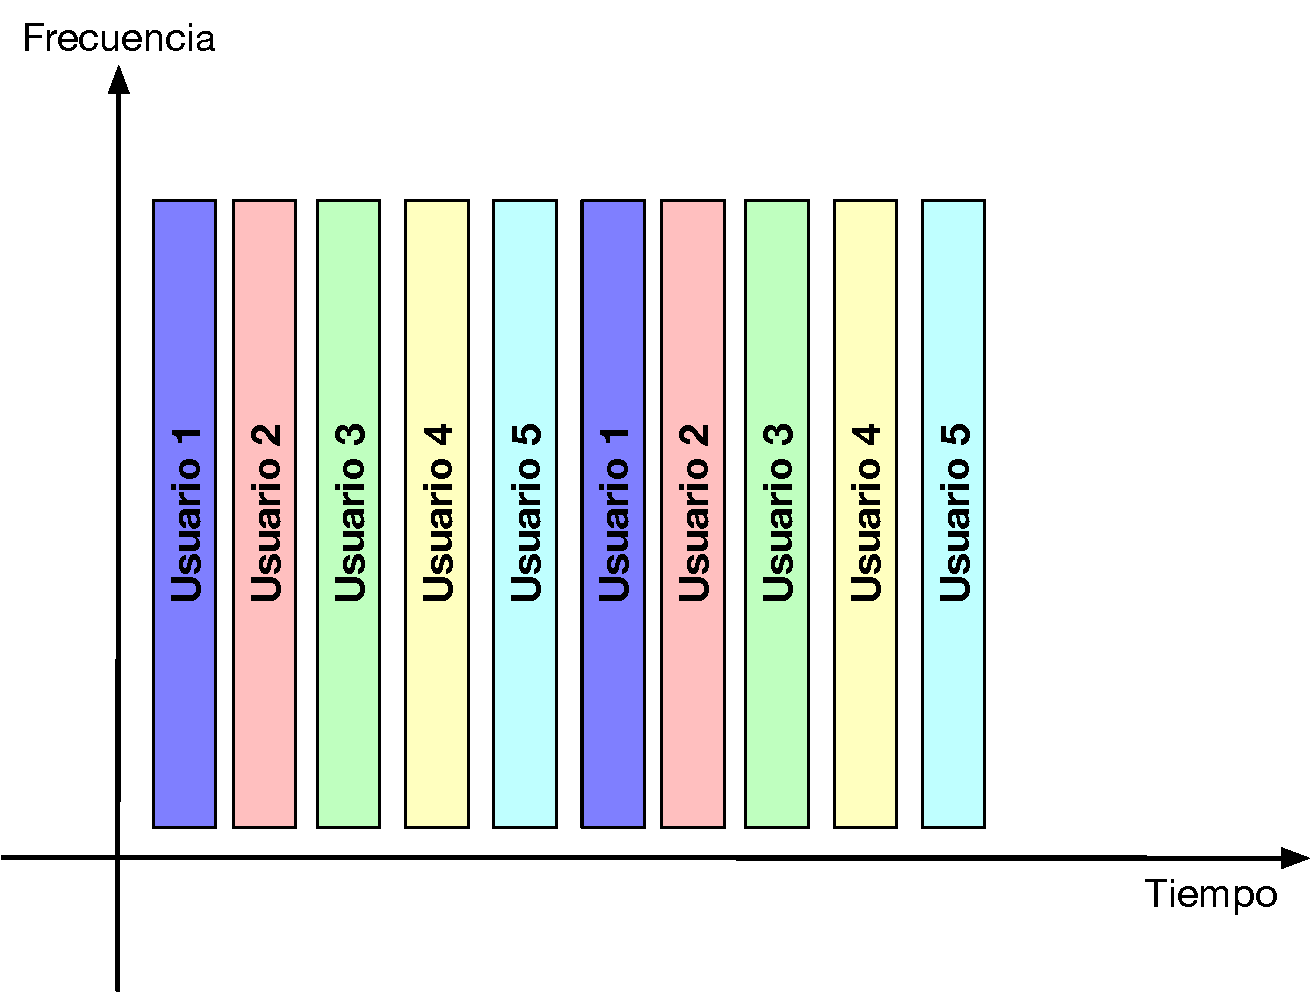
\includegraphics[width=8cm]{./Figuras/TDMA}
	\caption{Sistema TDMA.}
	\label{fig:TDMA}
\end{figure*}


Entre las ventajas de los sistemas TDMA podemos citar:

\begin{itemize}
	\item Versatilidad. Se pueden asignar más o menos slots a cada usuario en función de sus necesidades. 
	\item Buen rendimiento espectral.
\end{itemize}

Por otra parte, los principales inconvenientes de este tipo de técnicas son:

\begin{itemize}
	\item Complejidad, ya que se requiere una sincronización estricta para evitar colisiones. 
	\item Técnicas limitadas a sistemas digitales.
\end{itemize}
xº

Estas técnicas se utilizan, en combinación con FDMA, en los sistemas de telefonía móvil de 2ª generación (GSM). 

%%%%%%%%%%%%%%%%%%%%%%%%%
\subsection{Ejemplo: GSM}\index{GSM}
%%%%%%%%%%%%%%%%%%%%%%%%%

Como acabamos de decir, los sistemas de telefonía móvil de 2ª generación utilizan una combinación de FDMA y TDMA en su diseño. 

El enlace ascendente (del terminal a la estación base) utiliza las frecuencias entre 890 y 915 MHz, mientras que el descendente (de la estación base al terminal) usa la banda entre 935 y 960MHz. Cada banda de 25MHz acomoda un total de 125 portadoras o canales cada uno con un ancho de banda de 200kHz, y con 8 usuarios por canal, lo que hace un total de 1000 usuarios posibles.

Cada usuario transmite un bloque de datos cada 4,615ms, cada uno con una duración de 576,92$\mu s$, que equivalen a 156,25 bits. 

GSM también utiliza una técnica de saltos en frecuencia pseudoaleatorios, para evitar posibles problemas de desvanecimientos selectivos en frecuencia, de forma que la frecuencia de cada portadora cambia a un ritmo de 217 saltos por segundo. 
 
 \begin{figure*}[h!]
	\centering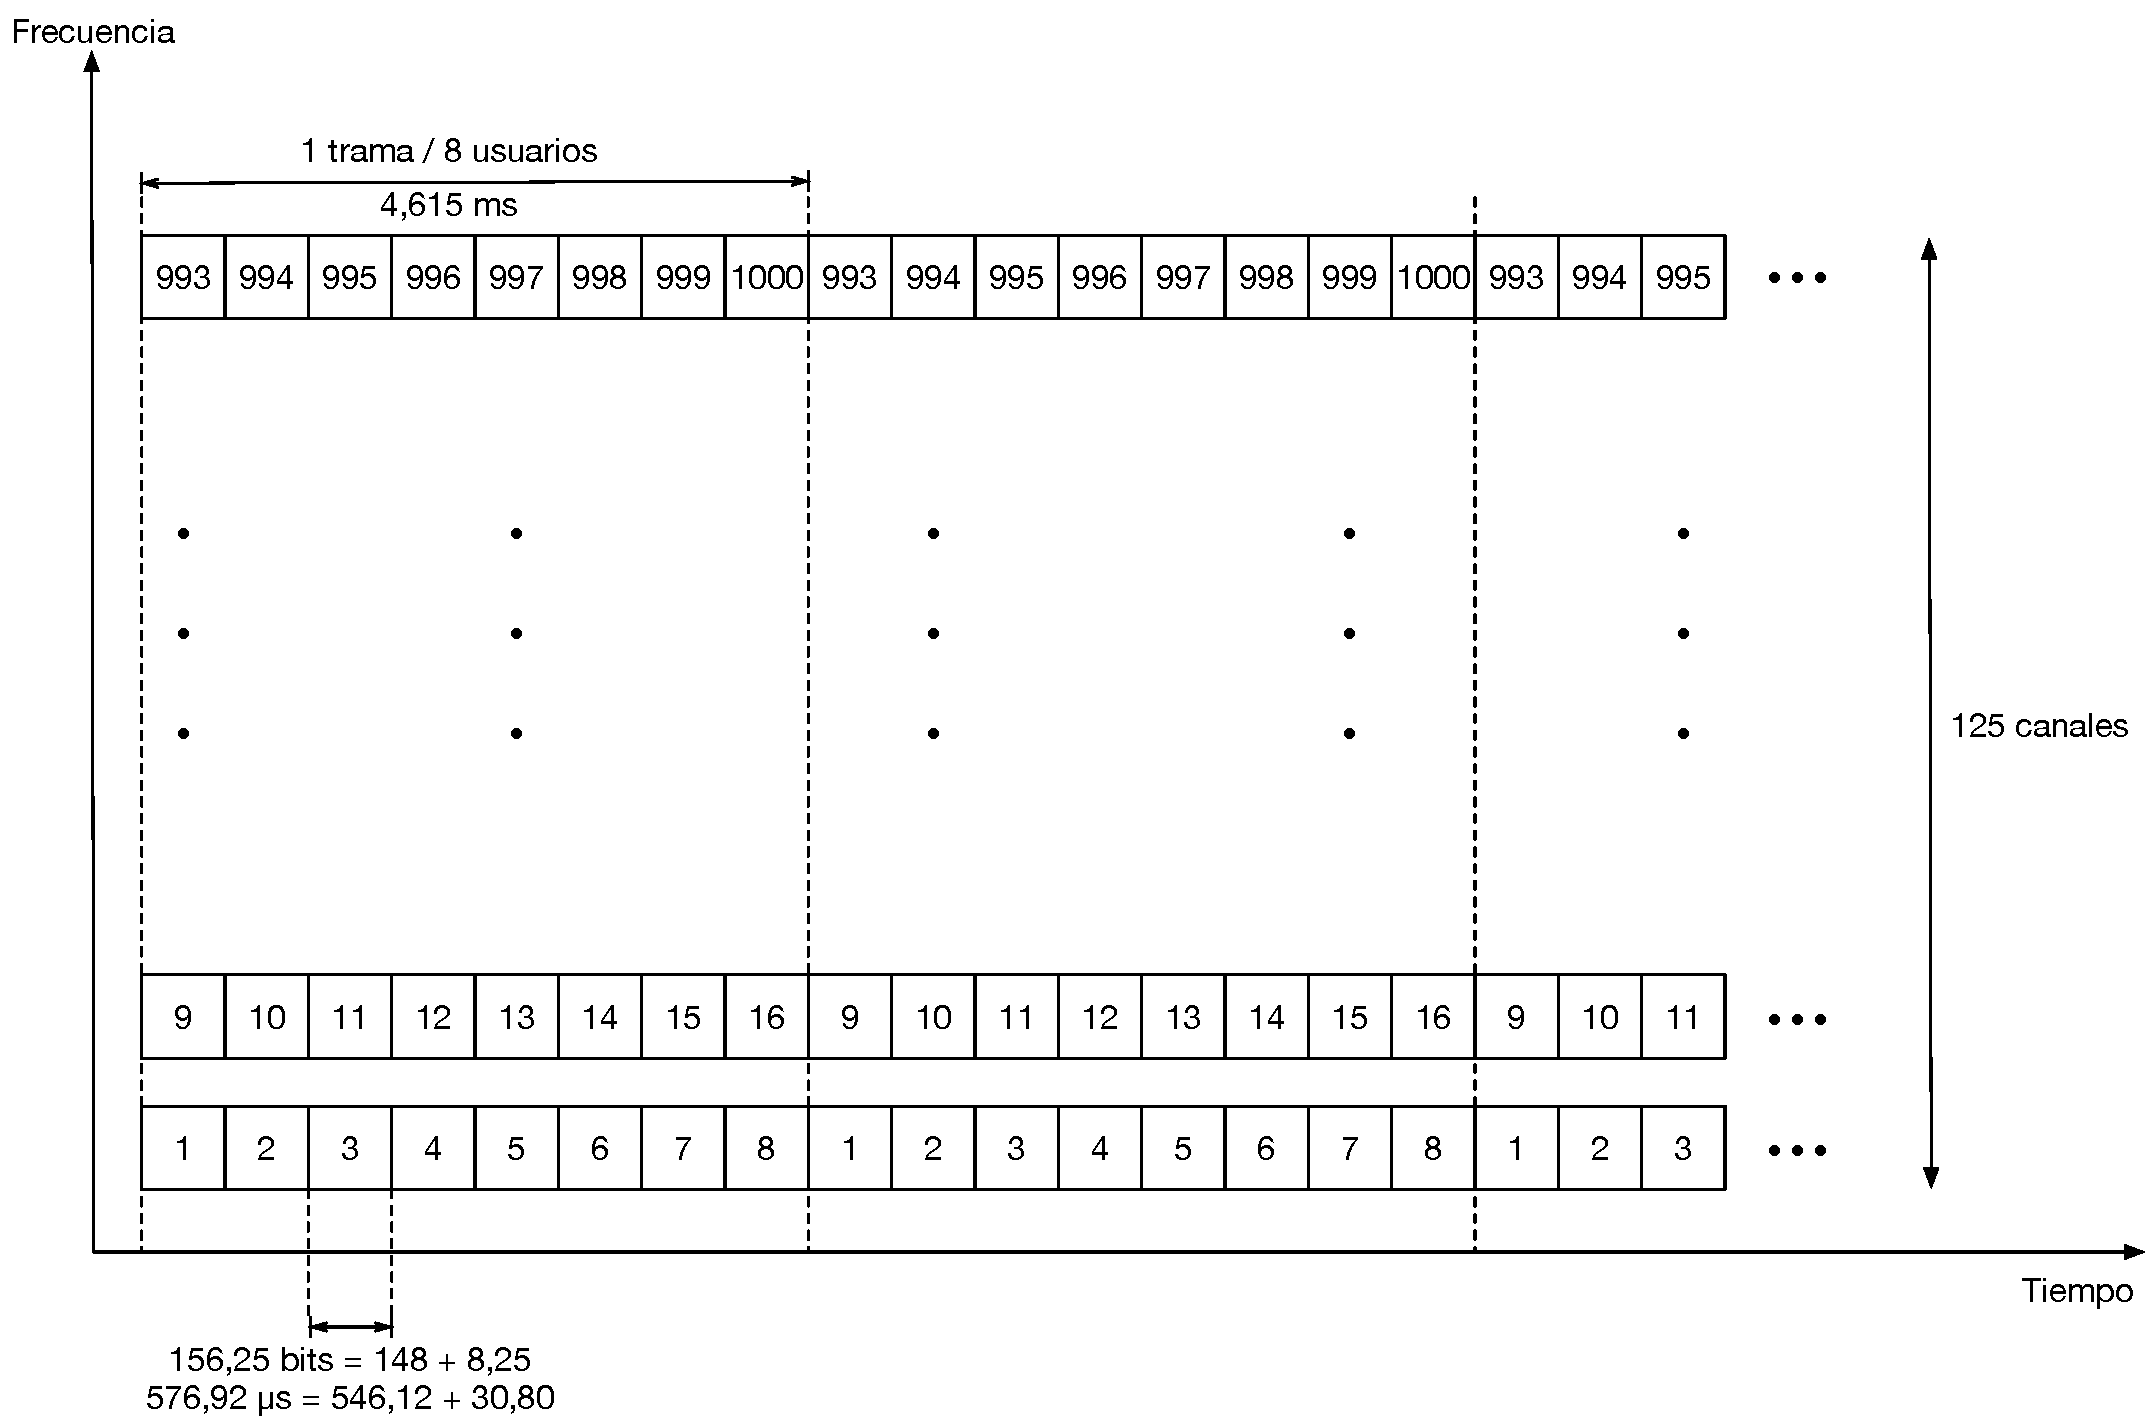
\includegraphics[width=10cm]{./Figuras/AccesoAlMedioGSM}
	\caption{Esquema de las técnicas de acceso al medio TDMA/FDMA en GSM.}
	\label{fig:AccesoAlMedioGSM}
\end{figure*}

 \begin{figure*}[h!]
	\centering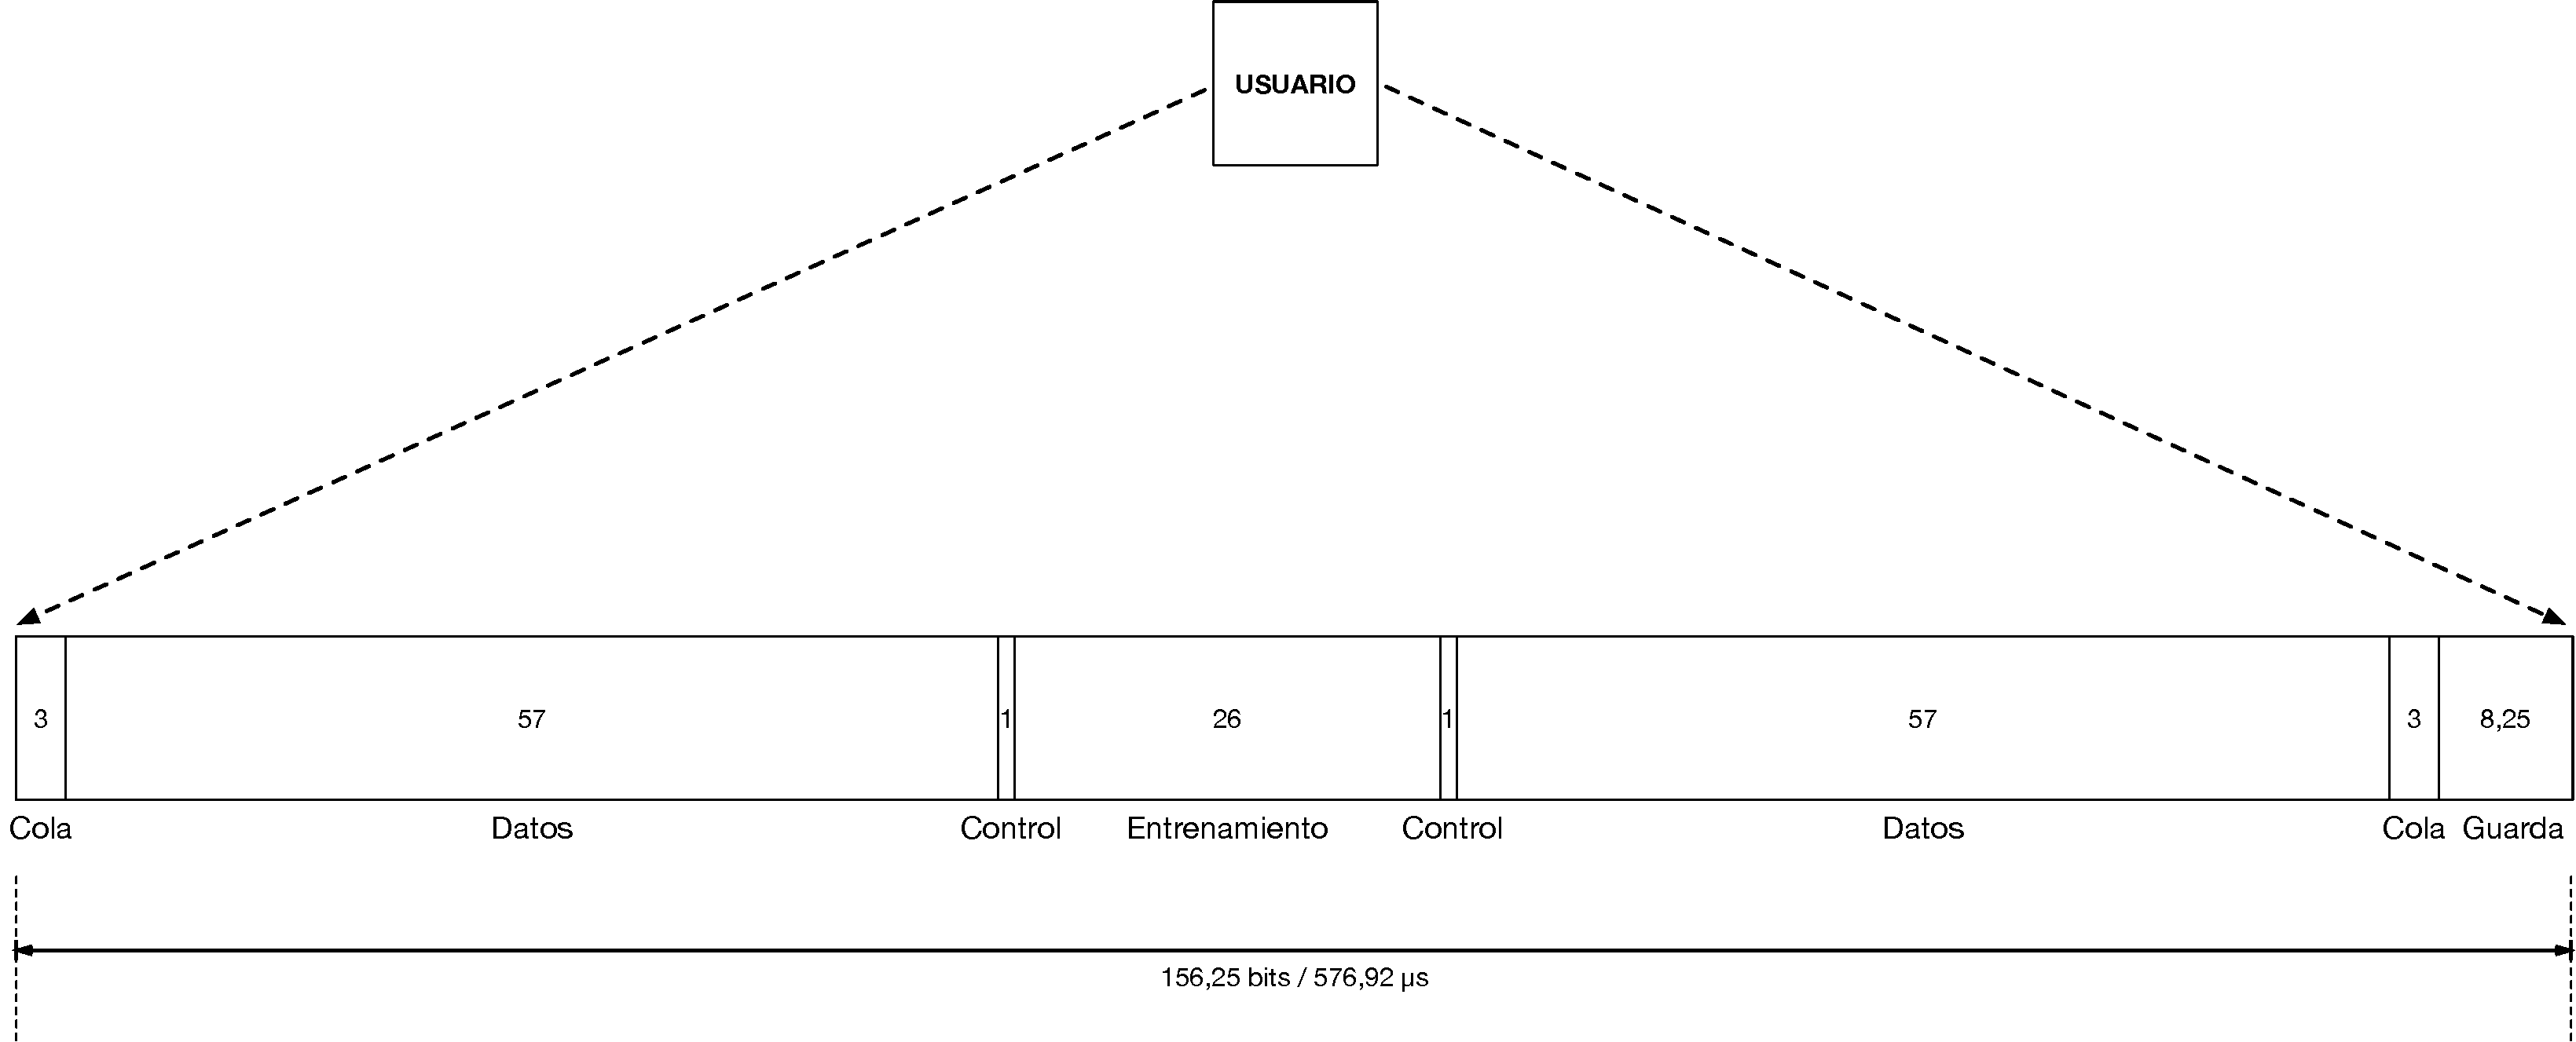
\includegraphics[width=10cm]{./Figuras/TramaGSM}
	\caption{Esquema de una trama GSM.}
	\label{fig:TramaGSM}
\end{figure*}
 
 %%%%%%%%%%%%%%%
\section{OFDMA}\index{OFDMA}\index{Orthogonal Frequency Division Multiple Access}
%%%%%%%%%%%%%%%

Hemos visto antes, cuando hablábamos de las técnicas FDMA, que a cada usuario se le asigna una portadora con un ancho de banda específico de forma que se pueda compartir el ancho de banda total del canal entre todos los usuarios. El mayor problema de esta técnica de acceso al medio era la posibilidad de interferencia entre subcanales, algo que, si se quiere evitar, requiere el uso de filtros paso banda muy exactos, y con ello costosos. 

Otra forma de intentar evitar la aparición de interferencia entre subcanales es hacer uso de pulsos de transmisión ortogonales que pueden solaparse total o parcialmente. Esto quiere decir que, si $f_k$ y $f_i$ son dos portadoras, se cumple que:

\begin{displaymath}
	\int_0^T \cos (2 \pi f_k t) \cos (2 \pi f_i t) = 0 \quad \forall k \neq i
\end{displaymath}

 De esta forma los distintos espectros se pueden solapar, y se evita el uso de los filtros paso banda necesarios en los sistemas FDMA convencionales. A este tipo de modulación se le denomina Acceso al Medio por División en Frecuencia Ortogonal (\emph{Orthogonal Frequency Division Multiple Access}, OFDMA).
 
 Por contra, OFDMA necesita que haya un mecanismo de sincronización muy estricto.
 
 En la Figura \ref{fig:OFDM} se representa un ejemplo del espectro de 8 señales OFDM. Con línea de puntos se muestran cada una de las señales individuales y en línea continua la forma que tendría el espectro global, suma de todos los anteriores.


\begin{figure*}[h!]
	\centering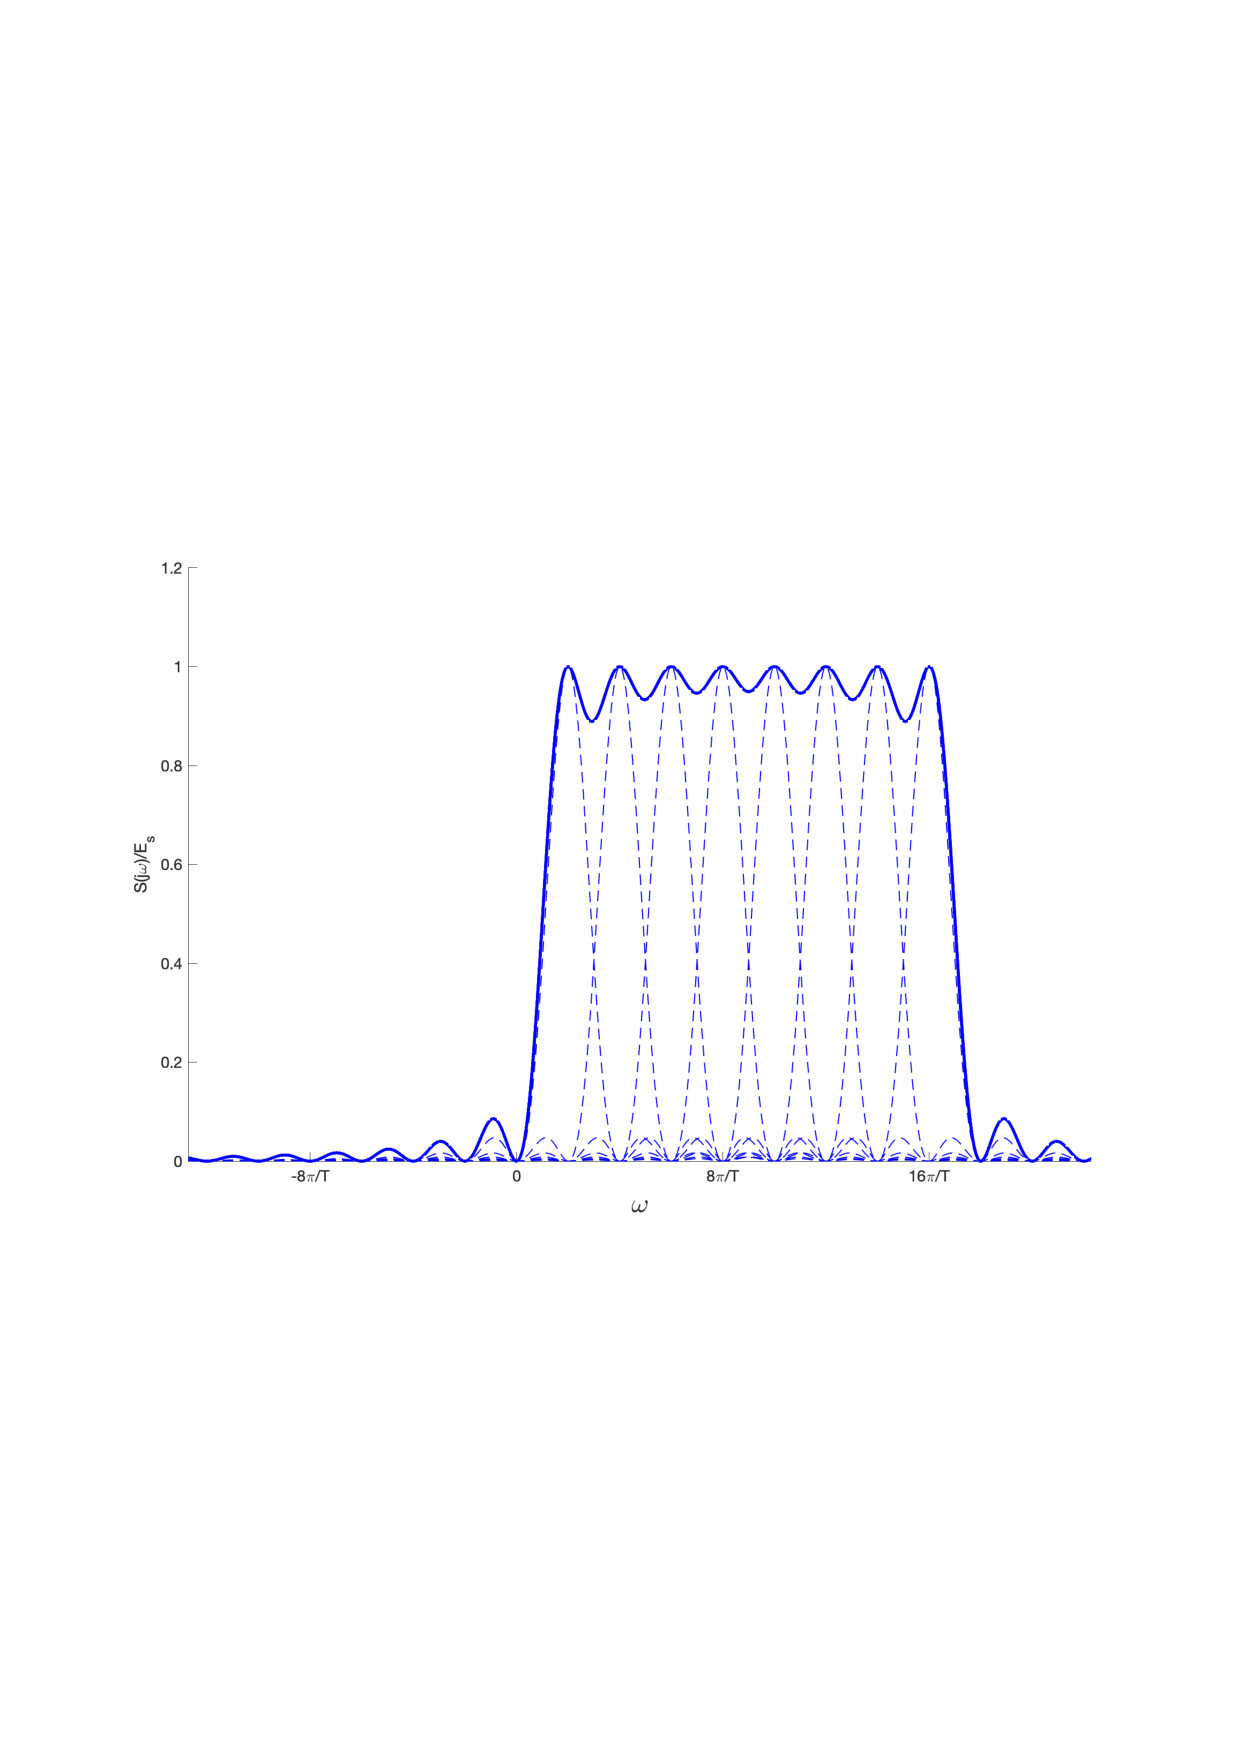
\includegraphics[width=12cm,height=6cm]{./Figuras/OFDM.pdf}
	\caption{Espectro de una señal OFDM con $N=8$. Se muestra cada uno de los espectros de los canales individuales en línea discontinua y el completo en línea continua.}
	\label{fig:OFDM}
\end{figure*}


Algunas de las aplicaciones más conocidas de este tipo de técnicas es en las redes inalámbricas Wi-Fi\index{Wi-Fi} (IEEE 802.11)\index{IEEE 802.11} o WiMax (IEEE 802.16)\index{WiMax}\index{IEEE 802.16}.

Es posible demostrar, utilizando el criterio de Nyquist generalizado, que si se dispone de un ancho de banda de $W$ Hz, se puede garantizar la existencia de pulsos de transmisión ortogonales suficientes como para dar servicio a $2WT$ usuarios. Esta cifra puede resultar demasiado baja en muchas aplicaciones reales, y la podemos aumentar si tenemos en cuenta dos ideas:

\begin{itemize}
	\item En muchos casos no es necesario asignar a un usuario un pulso de transmisión de forma permanente, ya que el tráfico se produce a ráfagas. Pensemos por ejemplo en una conversación telefónica, donde cada interlocutor está inactivo la mayor parte del tiempo. Podríamos aprovechar ese tiempo ``vacío'' para que otros usuarios transmitan, y para eso se han desarrollado multitud de técnicas como los métodos de escucha y detección de colisiones (CSMA/CD, \emph{Carrier Sense Multiple Access with Collision Detection})\index{CSMA/CD}\index{Carrier Sense Multiple Access with Collision Detection} que se usan en las redes Ethernet, los de paso de testigo (\emph{token}), etc. Este tipo de técnicas se encuentran en una capa superior a la física en la que nos estamos centrando en este texto, por lo que no vamos a profundizar más en ellas. 
	\item Una segunda alternativa consiste utilizar señales no ortogonales, pero sí ``casi'' ortogonales. De esta forma podremos incrementar el número de usuarios por encima del límite marcado por el criterio de Nyquist generalizado aunque a costa de la aparición de una interferencia multiacceso (MAI, \emph{Multi Access Interference})\index{MAI}\index{Multi Access Interference}. La ventaja es que se puede prescindir de las técnicas de asignación dinámica discutidas en el punto anterior, ya que todos los usuarios van a poder transmitir al mismo tiempo. Para hacer esto se recurre a las denominadas técnicas de espectro ensanchado, y surge así el siguiente tipo de técnica de acceso al medio que veremos: el acceso múltiple por división de código (CDMA, \emph{Code Division Multiple Access}).
\end{itemize}

 

%%%%%%%%%%%%%%%
\section{CDMA}\index{CDMA}\index{Code Division Multiple Access}
%%%%%%%%%%%%%%%

Para comprender mejor las técnicas de acceso al medio por división de código (CDMA) debemos antes describir las técnicas de espectro ensanchado\index{Espectro ensanchado}, pensadas inicialmente para reducir la sensibilidad a interferencias o para aumentar la privacidad en un sistema de comunicaciones. 

Existen distintas maneras de generar una señal de espectro ensanchado. Nosotros nos vamos a centrar en las técnicas de secuencia directa (DS, \emph{Direct Sequence})\index{DS}\index{Direct Sequence}\index{Secuencia directa}, que son las que se utilizan normalmente en los sistemas CDMA. No obstante, más adelante veremos también a modo de curiosidad algún otro ejemplo. 

Los sistemas de espectro ensanchado basados en secuencia directa\index{DS-CDMA} utilizan una secuencia pseudoaleatoria para multiplicar a la señal original de forma que se aumente su ancho de banda, haciendo que su espectro se expanda. En la figura \ref{fig:DS-CDMA} se muestra un esquema de cómo funcionaría un sistema de este tipo. La señal de entrada, que tiene un periodo de símbolo $T$ se multiplica por otra señal, llamada \emph{código}, formada por una serie de pulsos rectangulares llamados \emph{chips}, y cuyo periodo de símbolo es muy inferior, $T_c \ll T$. Esto produce una señal que tiene un ancho de banda muy superior al de la señal original, y que si se vuelve a multiplicar por el mismo código original, permite obtener de nuevo la señal con el mensaje. Todo este proceso se muestra de forma gráfica en la Figura \ref{fig:DS-CDMA}.


\begin{figure*}[h!]
	\centering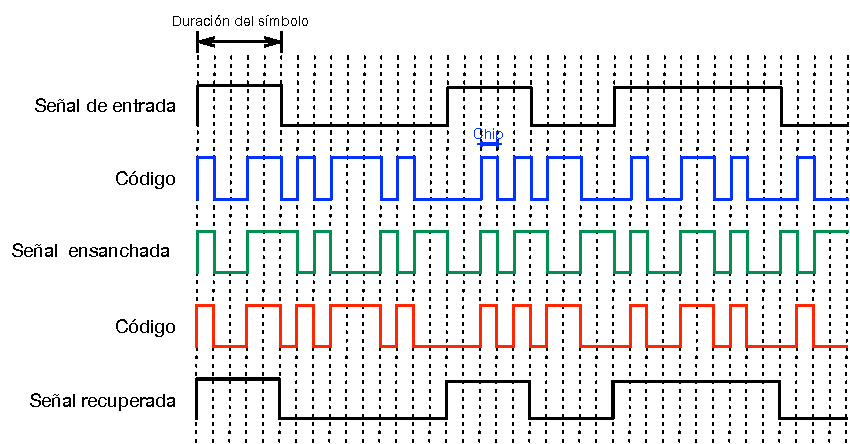
\includegraphics[width=10cm]{./Figuras/DS-CDMA}
	\caption{Sistema DS-CDMA.}
	\label{fig:DS-CDMA}
\end{figure*}

La señal de espectro ensanchado, para cualquier otro receptor que no disponga del código correcto, no tendrá ningún sentido, y se confundirá con el ruido de fondo del canal. 

Teniendo esta idea en mente, podemos pensar ahora en la situación en la que varios usuarios de espectro ensanchado comparten el mismo canal, utilizado cada uno su propio código. En este caso todos los usuarios van a transmitir simultáneamente en las mismas frecuencias. Para cada usuario, las transmisiones de los demás usuarios se ven como ruido, y si los códigos están bien diseñados, de forma que la correlación cruzada entre ellos sea mínima (aunque no tiene por qué ser cero, como hemos visto antes), la interferencia será mínima. Esto es precisamente un sistema CDMA. 


\begin{figure*}[h!]
	\centering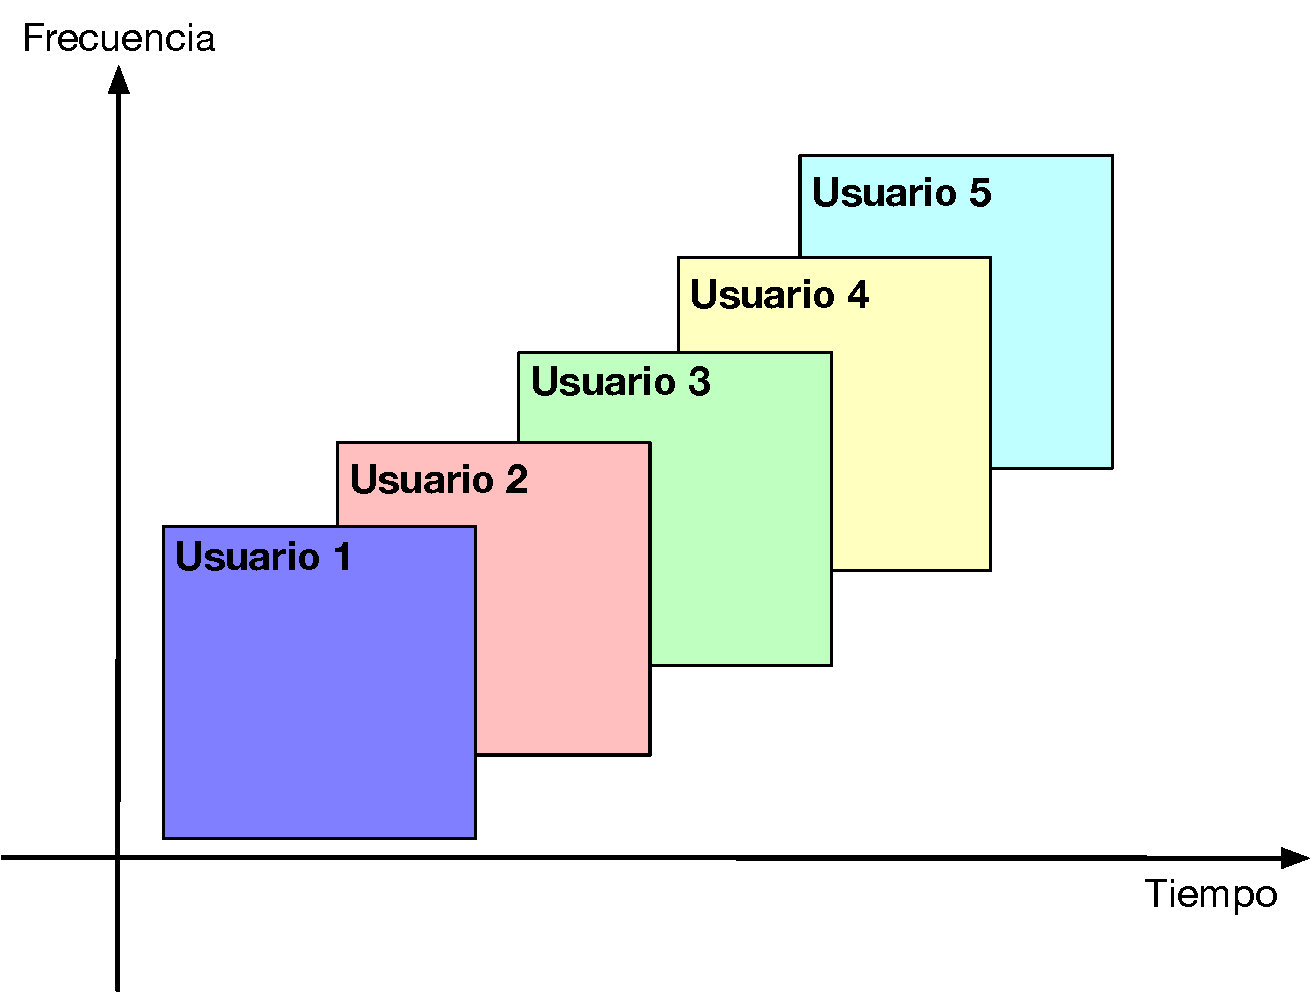
\includegraphics[width=7cm]{./Figuras/CDMA}
	\caption{Sistema CDMA.}
	\label{fig:CDMA}
\end{figure*}

Es posible demostrar que la probabilidad de error para un sistema CDMA con $M$ usuarios viene dada por\index{CDMA!Probabilidad de error}:

\begin{displaymath}
	P_e = Q \left ( \frac{1}{\sqrt{\frac{M-1}{3P_g} + \frac{N_0}{2E_b}}} \right )
\end{displaymath}

donde el parámetro $P_g$ se denomina ganancia del proceso y representa el cociente entre el ancho de banda de la señal expandida y el original: $P_g = W_c/W_x$. Fijándonos en la expresión anterior, podemos ver qué sucedería si el canal no introdujese nada de ruido:

\begin{displaymath}
	P_e = Q \left ( \sqrt{\frac{3 P_g}{M-1}} \right )
\end{displaymath}

Es decir, incluso para el caso de que el canal no introduzca nada de ruido, la probabilidad de error es no nula por el simple hecho de que haya otros usuarios en el sistema. Dicho de otro modo, mientras que para los sistemas FDMA o TDMA la presencia de más usuarios produce la aparición de problemas de interferencia entre subcanales, aquí lo que sucede es que aumenta el nivel de ruido de fondo. 

Ventajas del CDMA:

\begin{itemize}
	\item Las señales transmitidas tienen una densidad espectral de potencia baja, ya que la potencia se distribuye entre toda la banda de frecuencias. Por tanto, afecta poco a otros sistemas. 
	\item Privacidad: cada usuario tiene asignado un código pseudoaleatorio desconocido para los demás. 
	\item Cada cliente puede transmitir cuando quiera, sin necesidad de esperar a ningún \emph{slot}.
	\item Utilización más eficiente de todo el espectro.
\end{itemize}

Desventajas:

\begin{itemize}
	\item El rendimiento del sistema se degrada a medida que aumenta el número de usuarios. 
	\item Es un sistema limitado por interferencia. Esto significa que necesita un algoritmo de control de la potencia, lo que añade complejidad.
\end{itemize}

En cuanto a sus aplicaciones, quizás la más conocida es que esta es la técnica de acceso al medio utilizada en telefonía móvil 3G-UMTS.

\subsection{El problema cerca-lejos}\index{Cerca-lejos}\index{Problema cerca-lejos}

Uno de los principales problemas de los sistemas CDMA es el conocido como cerca-lejos. Esto se produce cuando al receptor le llegan señales de varios transmisores con distinta potencia. Un caso típico de esta situación es en los sistemas de telefonía móvil, donde cada usuario puede estar a una distancia distinta de la estación base, y por tanto su señal le llegará a ésta con una potencia distinta. 

Lo que sucede en este caso es que puede que el receptor tenga problemas para detectar la señal de un receptor con poca potencia cuando está en presencia de otras transmisiones con mucha mayor potencia. Una de las formas de solucionar este problema es implementar técnicas de control de potencia, de forma que cada transmisor ajuste su potencia transmitida para asegurar que todos lleguen al receptor con una relación señal a ruido similar. Esto además permite ahorrar batería en terminales móviles, ya que pueden reducir la potencia a la que transmiten cuando están cerca de su estación base. 

\subsection{CDMA con saltos en frecuencia}\index{Saltos en frecuencia}\index{FH}\index{Frequency Hopping}

Como decíamos antes, existe una segunda forma de obtener señales con espectro ensanchado, que tiene un curioso origen en los años previos a la Segunda Guerra Mundial. Fue entonces cuando la actriz Hedy Lamarr ideó, junto con el compositor George Antheil, una técnica para controlar los torpedos a distancia que era inmune a los sistemas de detección del enemigo. La idea era que la señal de control del torpedo fuese saltando de una frecuencia a otra de una forma pseudoaleatoria que sólo conocería el receptor (el torpedo). Así nació la técnica de espectro ensanchado por salto en frecuencia (FH, \emph{Frequency Hopping}). 

Como acabamos de decir, la idea detrás de las técnicas de salto en frecuencia es dividir el espectro disponible en varias bandas de frecuencia sin solape. Así, la banda utilizada para enviar la señal a transmitir va variando de forma pseudoaleatoria. 

\begin{figure*}[h!]
	\centering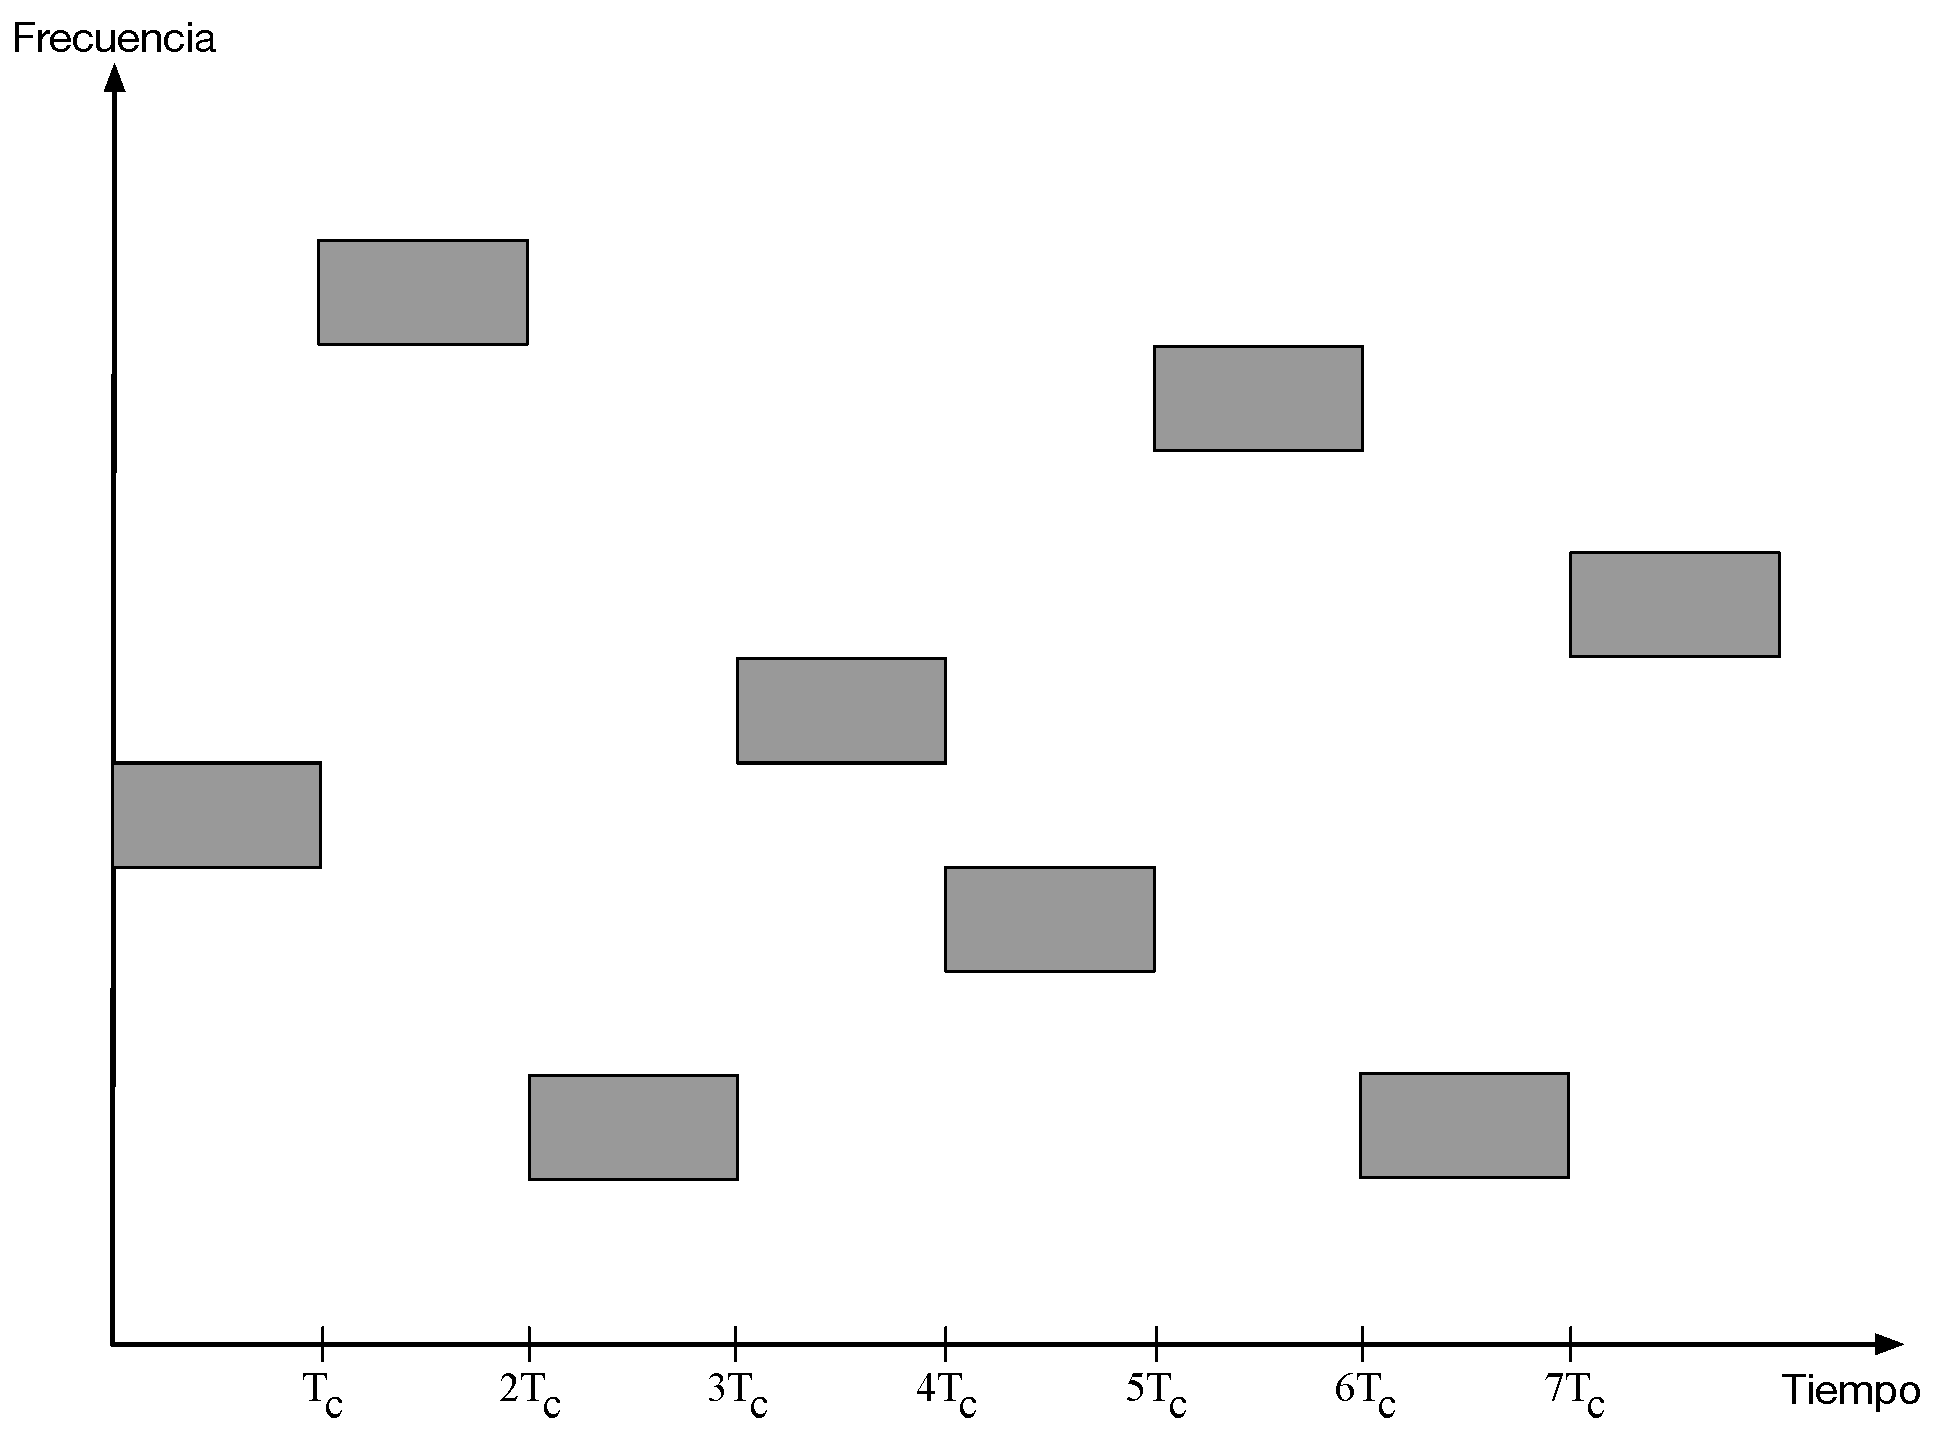
\includegraphics[width=7cm]{./Figuras/FrequencyHopping}
	\caption{Ejemplo de sistema de espectro ensanchado por saltos en frecuencia.}
	\label{fig:FrequencyHopping}
\end{figure*}

Se puede hacer que el periodo de los saltos en frecuencia sea menor o mayor que el periodo de símbolo. En el primer caso hablaremos de un sistema de {\bf saltos lentos en frecuencia}, mientras que en el segundo será un sistema de {\bf saltos rápidos en frecuencia}. 




%%%%%%%%%%%%%%%
\section{SDMA}\index{SDMA}\index{Spatial Division Multiple Access}
%%%%%%%%%%%%%%%

La técnica SDMA segmenta el espacio en distintos sectores dentro de cada uno de los cuales se utilizará alguna otra técnica de acceso. Los sistemas GSM, por ejemplo, utilizan SDMA en combinación con TDMA. Para conseguir esto se suelen utilizar por ejemplo antenas directivas, de forma que con distintos haces de radiación se cubren distintas zonas del espacio. 

%\begin{figure*}[h!]
%	\centering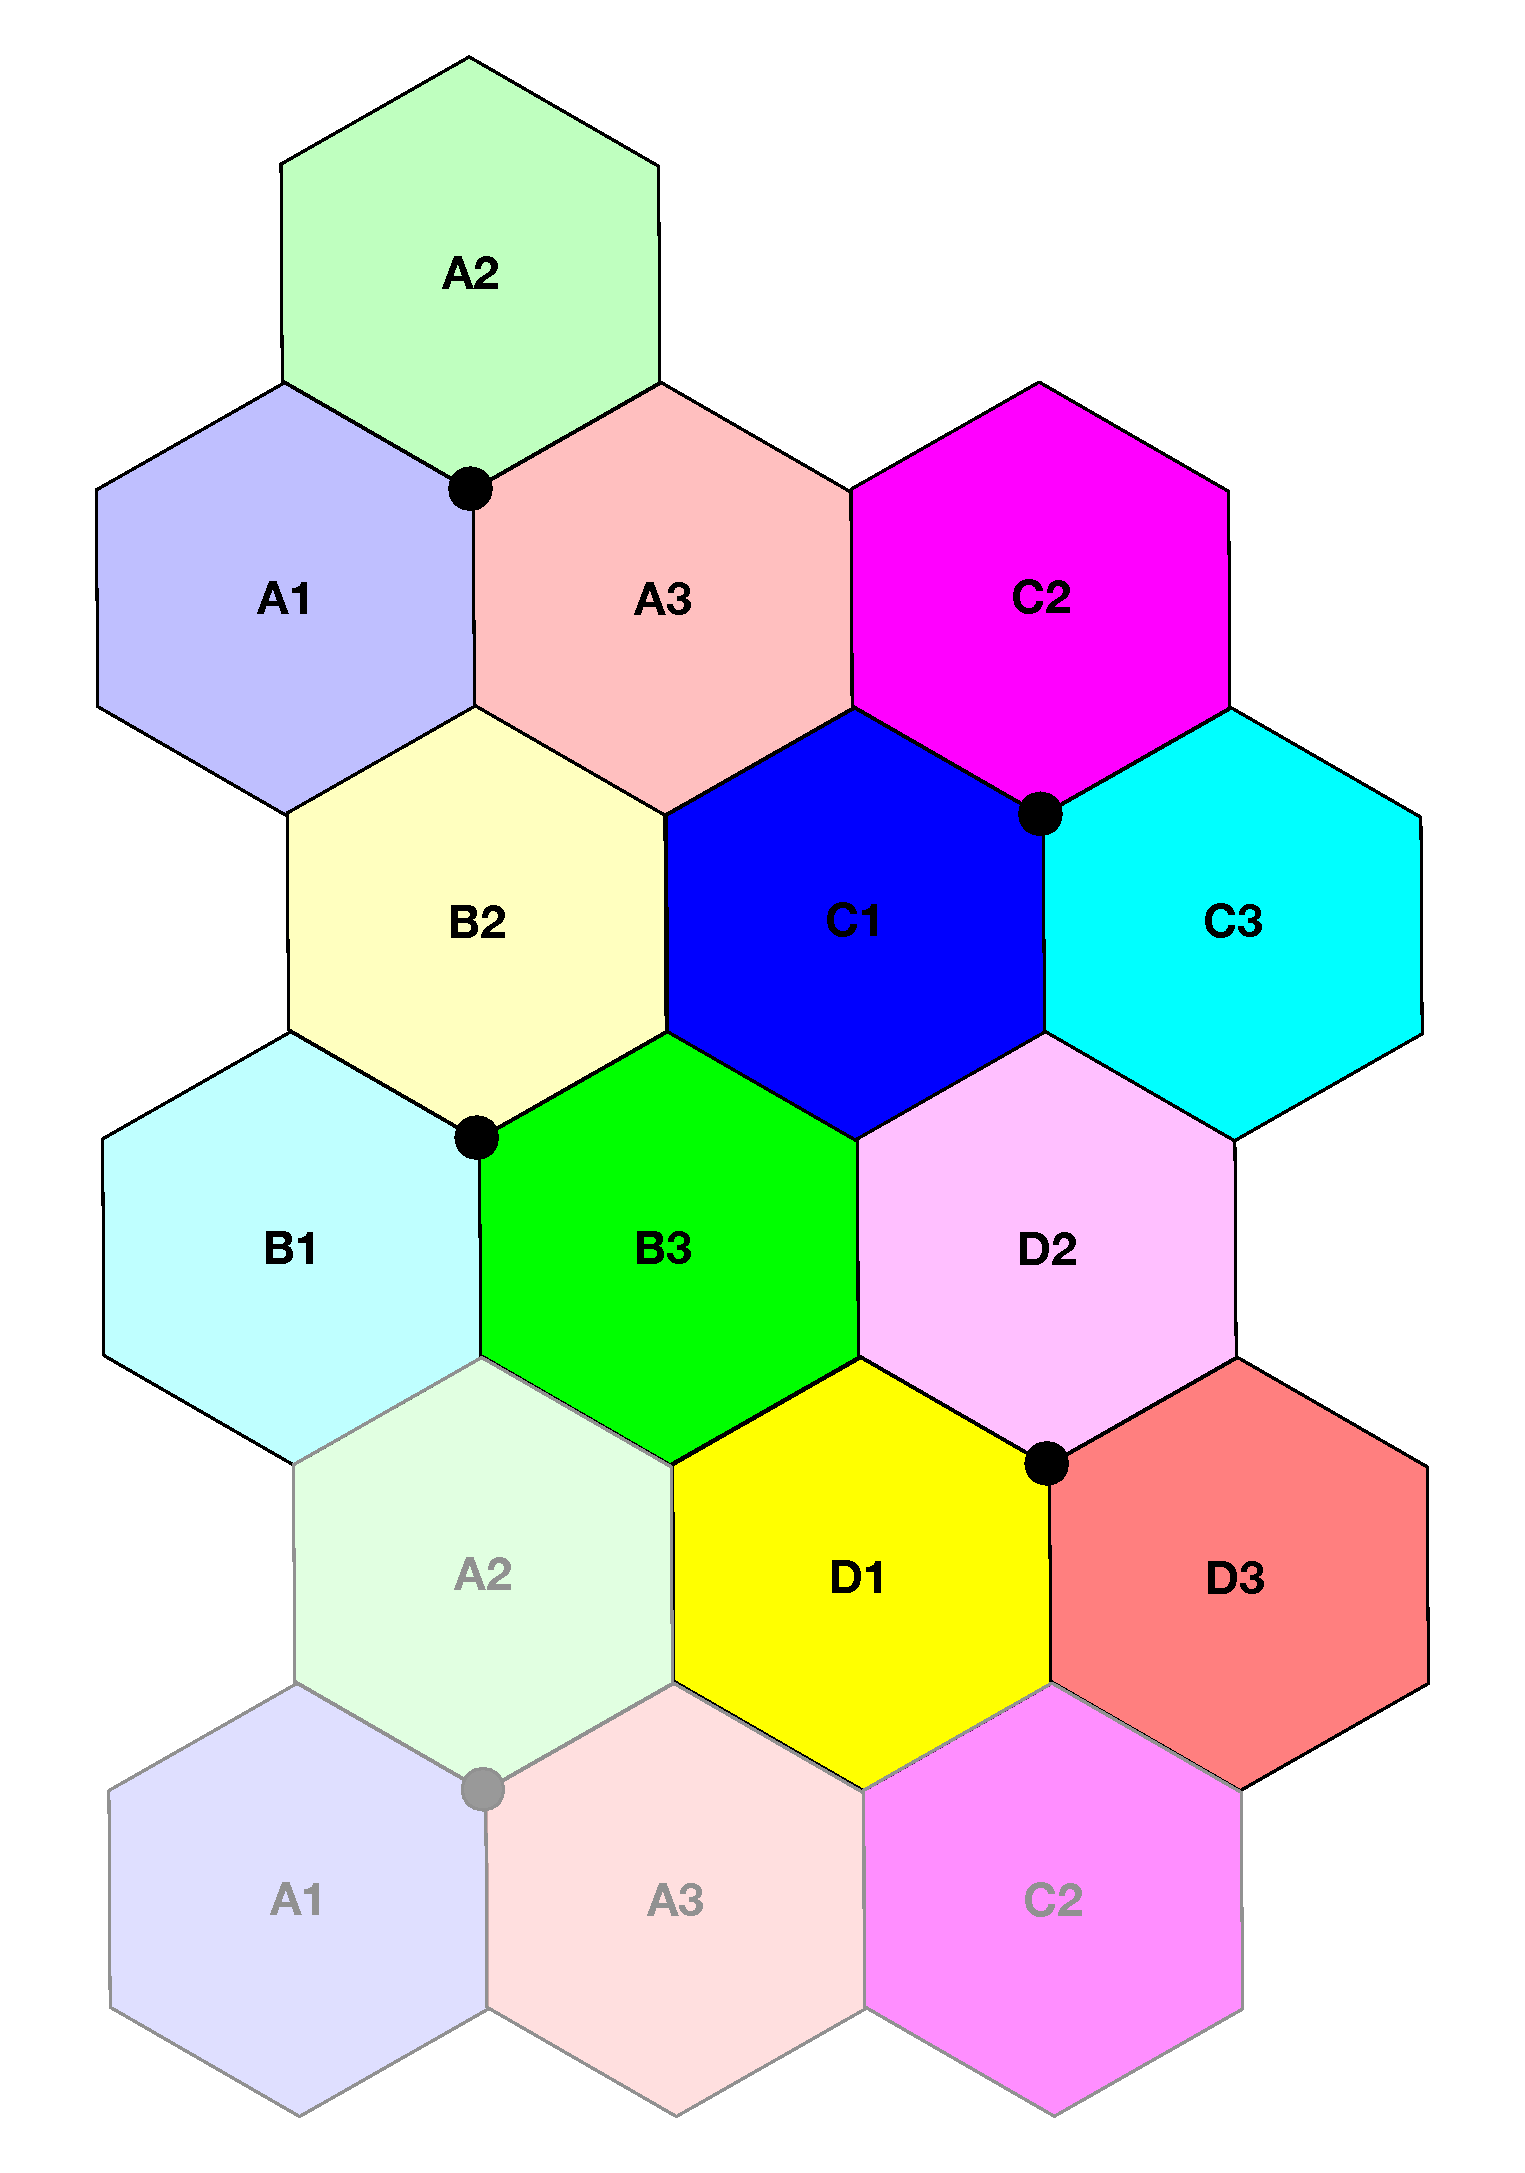
\includegraphics[width=7cm]{./Figuras/SDMA}
%	\caption{Sistema SDMA combinado con TDMA.}
%	\label{fig:SDMA}
%\end{figure*}


\section{Problemas propuestos}



\ProblemaBoletin{
	Se pretende diseñar un sistema FDMA para $10$ usuarios de forma que a cada uno de ellos se le asigne un canal de ancho de banda $W$. Se debe considerar además una banda de guarda entre canales $B_g$. Considerando que el módulo de la respuesta en frecuencia de los filtros paso banda viene dado por:
		\begin{displaymath}
			|H(f)| = e^{-\left ( 1.2 \frac{f-f_0}{W} \right )^2 }
		\end{displaymath}
		donde $f_0$ es la frecuencia central de cada uno de los canales. 
		Calcule el valor de $B_g$ de forma que se garantice que la respuesta entre canales adyacentes cumpla $|H(f) \leq 0.1$
		¿Cuál sería el ancho de banda global de todo el sistema FDMA?
	}
	{$B_g = 0.76 W$, $B=17W$.}{}{}

\ProblemaBoletin{
	Un sistema CDMA tiene $P_e = 10^{-7}$ y $P_g = 30dB$. ¿Cuántos usuarios adicionales puede admitir garantizando que $P_e \leq 10^{-5}$?
	
	\textsc{NOTA:} 
	\begin{displaymath}
			P_e = Q \left ( \frac{1}{\sqrt{\frac{M-1}{3P_g} + \frac{N_0}{2E_b}}} \right )
	\end{displaymath}
	}{
		54 usuarios en total
	}{}{}

	

\end{document}



	
